%! Author = abenjeddou
%! Date = 30/06/2026

\section{Introduction}
This chapter covers the third sprint, focused on implementing the notification delivery to the Erable push notification API and persisting the processing state back to Valkey.

\section{Sprint Goal}

For this sprint, we want to implement the notification delivery to the Erable push notification API and persist the processing state back to Valkey.

\section{Logical Pipeline Overview}

\begin{figure}[!htbp]
    \centering
    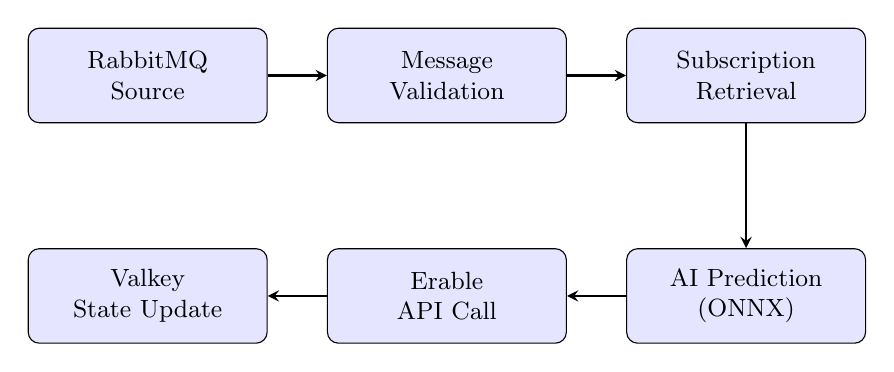
\begin{tikzpicture}[
        node distance=1.8cm,
        block/.style={rectangle, draw, fill=blue!10, text width=2.8cm, text centered, minimum height=1.2cm, rounded corners, font=\small},
        arrow/.style={->, >=stealth, thick}
    ]
        \node[block] (src) {RabbitMQ\\Source};
        \node[block, right of=src, xshift=2cm] (valid) {Message\\Validation};
        \node[block, right of=valid, xshift=2cm] (sub) {Subscription\\Retrieval};
        \node[block, below of=sub, yshift=-1cm] (ai) {AI Prediction\\(ONNX)};
        \node[block, left of=ai, xshift=-2cm] (erable) {Erable\\API Call};
        \node[block, left of=erable, xshift=-2cm] (sink) {Valkey\\State Update};

        \draw[arrow] (src) -- (valid);
        \draw[arrow] (valid) -- (sub);
        \draw[arrow] (sub) -- (ai);
        \draw[arrow] (ai) -- (erable);
        \draw[arrow] (erable) -- (sink);
    \end{tikzpicture}
    \caption{LFU job logical pipeline}
    \label{fig:logical-pipeline}
\end{figure}

\section{Erable API Call Operator}

The \texttt{LFUErableCallProcessFunction} sends the push notification to the Erable system via an HTTP POST call. It:
\begin{enumerate}
    \item Builds the \texttt{LFUErableEntity} containing the MSISDN, customer type, event type, and reached threshold.
    \item Sends the request via Spring \texttt{WebClient} with a configurable retry mechanism.
    \item Only forwards the message downstream if the response is \texttt{2xx}.
    \item Increments per-SID counters (OMOI, SOSH, OPRO) for successful sends.
\end{enumerate}

\begin{lstlisting}[language=Java, caption={HTTP call to Erable}]
LFUErableEntity body = buildEntity(fairUseMessage);
String erableUri = ErableCallUtils.getPath(
    erableCallConfiguration.getErableHost(),
    erableCallConfiguration.getErablePathPattern(), sid);

ResponseEntity<String> response = ErableCallUtils.sendErableRequest(
    client, erableUri, erableUuid, body,
    erableCallConfiguration, LOG);

if (response.getStatusCode().is2xxSuccessful()) {
    incrementOmoiOrSoshOrOpro(/* counters */);
    collector.collect(notification);
}
\end{lstlisting}

\section{Erable Error Handling}

\begin{itemize}
    \item \textbf{Automatic retry} via \texttt{ErableCallUtils.shouldRetry()} for transient errors (too many requests, connection timeouts, 5xx responses).
    \item \textbf{Critical errors} (e.g., repeated 5xx): exception propagation via \texttt{throwIfCriticalStatus()} to trigger a Flink restart.
    \item \textbf{Non-critical errors} (e.g., 4xx): log with code \texttt{UNMANAGED\_ERROR} + counter increment, message dropped.
    \item \textbf{Null response}: logged as \texttt{ERABLE\_ACCESS\_ERROR}, message dropped.
\end{itemize}

\section{State Update Sink}

The \texttt{LFUUpdateSubscriptionSink} class updates the \texttt{LfuMainRecord}'s state in Valkey with the timestamp of the last processed event. This enables the next processing cycle to compute the time interval since the last notification.

\begin{lstlisting}[language=Java, caption={State update in Valkey}]
lfuMainRecord.getState().setStates(
    Map.of(eventType, Map.of("last", timestamp)));
dao.updateLfuMainRecord(lfuMainRecord);
\end{lstlisting}

\texttt{DataPersistenceException} errors are caught, logged with code \texttt{PERSISTENCE\_LIB\_ ACCESS\_ERROR}, and the per-SID failed counter is incremented.

\section*{Conclusion}

At the end of Sprint~3, almost the full notification pipeline was functional end-to-end: messages were consumed from RabbitMQ, validated, enriched with subscription data, sent to Erable, and their state persisted in Valkey. The stub mode (\texttt{ERABLE\_STUBBED=true}) allowed testing without a live Erable instance.

